%# -*- coding: utf-8-unix -*-
% !TEX program = xelatex
% !TEX root = ../thesis.tex
% !TEX encoding = UTF-8 Unicode

\section{实体理解:实体链接任务}
\label{sec:rw-linking}


实体链接任务是一类从自然语言文本中识别出代表实体的字符串,
并将其映射到知识库中特定实体的任务。
人工进行的实体链接体现在维基百科的页面编辑过程中,
页面作者会手动为部分代表实体的短语添加超链接,
指向对应实体的维基页面。
这种带有维基内部超链接的短语被称为锚文本(Anchor Text),
本文中也称为实体短语。
基于机器学习的实体链接可以应用于不同场合的文本输入,
背后所使用的目标知识库也不局限于维基百科,
其它常用的知识库包括DBPedia,Yago以及Freebase。
考虑到这些知识库均基于维基百科信息构建而成,
实体链接任务又被称为``{维基化}'' (Wikification)
\cite{mihalcea2007wikify}。

以英文维基百科为例,一个典型的实体链接任务见下例:

\vspace{0.2cm}
%\begin{minipage}{0.5\columnwidth}
%\begin{center}
\underline{Michael Jordan}, also known by his initials, MJ, 
is a former professional \underline{basketball}
player. He played 15 seasons in the 
\underline{National Basketball Association} for 
the \underline{Chicago Bulls}
and \underline{Washington Wizards}.
%\end{center}
%\end{minipage}
\vspace{0.2cm}

实体链接任务首先需要提取出句中存在的实体短语,即下划线对应的部分。
该步骤与命名实体识别任务类似,
不同之处在于我们关注的实体短语除了命名实体
(具体的人名、地名、组织名、书名、电影名等)之外,
还包含了维基百科中存在的概念实体,用于指代一组相似实体。%例如森林、哺乳动物、运动员等。
下一个步骤对每个实体短语从维基百科中抽取出候选实体集,
并定义短语和候选实体之间的匹配分数,从而将短语链接至最相关的候选实体,
例如句中的5个实体短语分别对应维基百科中的实体
\textit{Michael Jordan}\footnote{https://en.wikipedia.org/wiki/Michael\_Jordan},
\textit{basketball}\footnote{https://en.wikipedia.org/wiki/Basketball},
\textit{National Basketball Association}\footnote{https://en.wikipedia.org/wiki/National\_Basketball\_Association},
\textit{Chicago Bulls}\footnote{https://en.wikipedia.org/wiki/Chicago\_Bulls}
以及\textit{Washington Wizards}\footnote{https://en.wikipedia.org/wiki/Washington\_Wizards}。

除了无结构的纯文本以外,互联网语料中的表格也蕴含了大量与实体相关的知识。
对表格进行实体链接的研究起源于Limaye等人\cite{limaye2010annotating}的工作,
如\figref{fig:rw-linking-limaye}所示,除了每个单元格所对应的实体之外,
得益于半结构化的组织形式,同一表列内的实体通常具有相同的类型,
而且两列实体之间描述了同一种关系的不同实例,
这些是非结构化文本所不具备的优势。
因为表格带来了丰富关系知识,表格上的实体链接在近年来受到了更多的关注。

\begin{figure}[th]
	\centering
    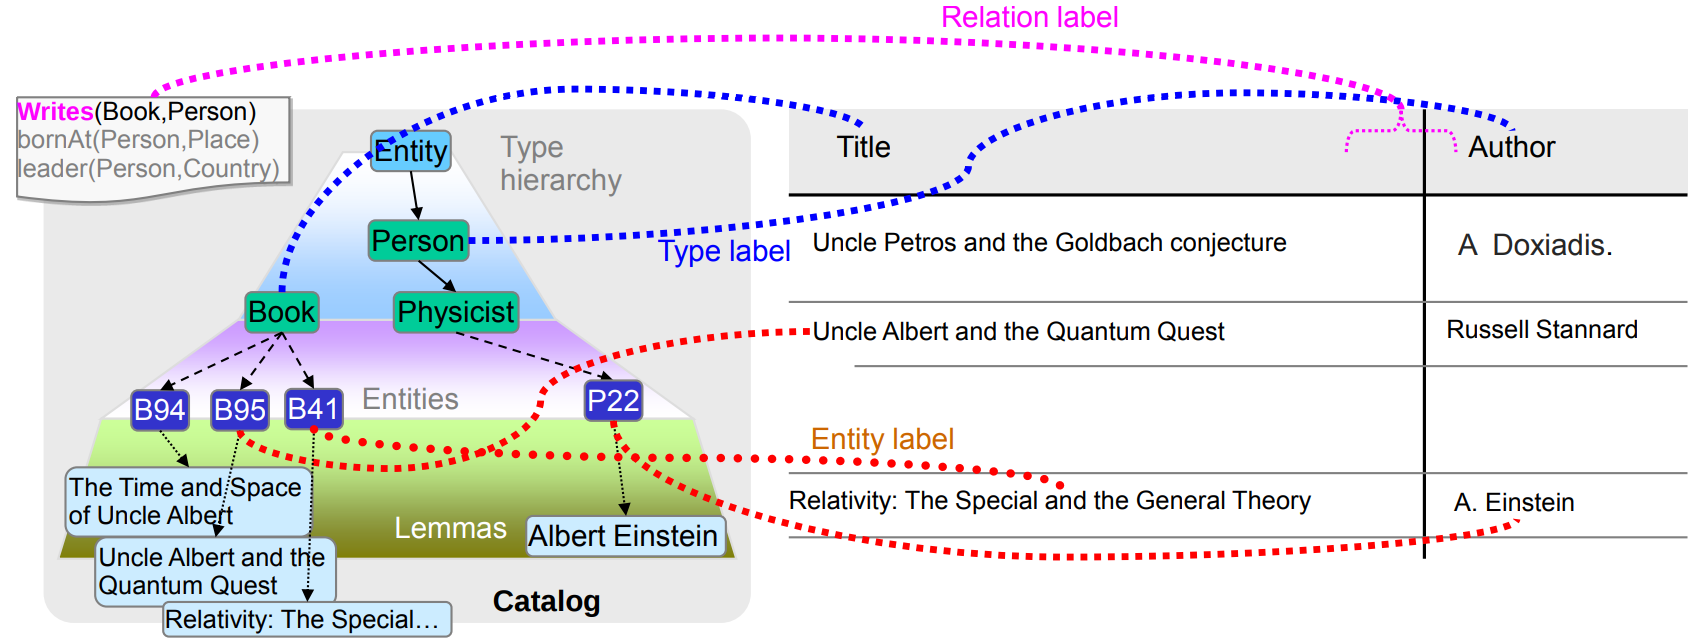
\includegraphics[width=0.95\columnwidth]{figure/rw/linking-limaye.png}
	\bicaption{Limaye等人提出的表格链接任务。\cite{limaye2010annotating}}{Entity linking task on web tables proposed by Limaye et al.}
	\label{fig:rw-linking-limaye}
\end{figure}

%讲一下和下游任务的联系,分别列举,从Han的变来
作为自然语言理解中的基本任务,实体链接是一系列下游任务的前置步骤。
%例如关系分类、阅读理解以及自动问答,
%(加上引用,有了论文就知道怎么聊)
%=============%
首先,开放式信息抽取抽取的主谓宾三元组均为文本表示,通常具有歧义,
一些研究工作旨在对三元组中的实体短语进行链接,
代表文献包括\parencite{nakashole2012patty,lin2012entity},
在实现三元组消歧的同时,结合知识库推理出主语和宾语所代表的类型,
有助于挖掘不同谓词关系之间的语义联系。
%=============%
其次,实体链接与知识库补全任务密切相关,
%带链接的关系三元组与知识库补全任务密切相关,
该任务的目的是向已有知识库中补充新的事实三元组。
这些新添加的三元组主要来源于两方面:
随时间发展所产生的全新事实,或基于已有知识的归纳推理。
基于前者的补全依赖于信息抽取系统的不断挖掘,
因此对主宾语的链接的准确率决定了知识库补全的效果。
知识库补全的相关内容将在\secref{sec:rw-kbc}中论述。
%=============%
最后,对于自动问答任务,%此处加cite?
尤其是我们关注的基于知识库的事实类自动问答任务,
其描述的是与问句中实体相关的事实,
因此不管以何种方式对答案进行建模,都依赖于对已有实体的准确定位,
以限定问句对应语义的搜索范围。
%=============%
%Information Retrieval以及Context Analysis
%都是非常重要的子任务
%实体链接结果给句子提供了知识库维度上的特征,
%并且限定整句的语义范围。
因此,实体链接的结果好坏,对这些任务的效果均有着很大程度的影响。
%常用的数据集包括xxxxx,以及表格数据集xxx

%以下是实体链接任务中的主要数据集。
%TAC-KBP\cite{}是xxxx,包含了xxxx的xxxx。
%AIDA数据集\cite{}由Hoffart等人提出,包含了。。。。
%Web Manual数据集\cite{}
%此外还有相关语料库,例如FACC1\cite{}...
%数据集:(Tutorial71-77)

实体链接的重点在于从多个候选中找出正确的那个实体,
其本质为消除实体级别存在的一词多义性,
例如短语 ``Michael Jordan'' 具有多个可能的候选,
在维基百科中可能代表篮球明星、足球运动员、著名的机器学习教授,
甚至更多不那么有名的人。
在缺乏上下文信息的情况下,很难进行准确的链接。
因此,一个良好的实体链接模型,相关性分数需要考虑多个因素,
包括实体本身的先验知识,实体与短语的匹配程度,以及实体与短语所在上下文的契合度。

基于特征工程的方式,其信息来源主要为维基百科上的统计数据。
随着深度学习的发展,
实体链接的研究将重心放在用表示学习替代或改良传统的特征工程方法。
得益于也文本的向量表示技术,以及神经网络的特征学习能力,
深度学习方法通过计算文本、实体的向量作为其语义表达,
并利用高维空间的相似度衡量短语和候选实体之间的相关性,
在效果上也取得了不错的提升。
接下来的几个小节主要介绍基于特征工程和深度学习的实体链接模型,
并单独介绍用于跨语言链接场景中的跨语言词向量技术。


\subsection{基于特征工程的实体链接}
\label{sec:rw-linking-feature}

基于特征工程的实体链接方法,较为经典的工作包括文献
\parencite{hoffart2011robust,ratinov2011local,shen2012linden,yang2015s,luo2015joint}。
这类方法的共性在于用预定义好的函数或概率值,
描述候选实体与实体短语及其上下文之间的特征,
通过学习特征的带权相加计算最终的匹配度。


在这类方法中,一个候选实体所具有的特征可以分为三类:
先验特征,上下文语义特征,以及与句中其它实体的关联特征。
%=======================%
先验特征与短语所处的文本无关,
仅基于短语与候选实体在维基百科中的统计信息,
主要体现为短语所在锚文本链接至该实体的概率,
以及实体出现在不同维基页面中的概率。
%=======================%
上下文语义特征关注文本及目标实体的语义近似程度,
利用词袋模型(Bag-of-Words)将短语的上下文
以及目标实体的维基页面分别转化为向量形式,
通过TF-IDF得到不同词语的重要性,
并用向量间的相似度
%(余弦相似度,点积或KL散度)
代表语义匹配程度。
%=======================%
实体间的关联特征体现在不同短语所对应的实体之间,
它们维基百科页面的相关性有助于实体链接的判断。
在维基百科中,若两个实体同时指向的页面较多,
或同时指向这两个实体页面的其它实体较多,
则它们具有较高的相关度。
常用的计算方式主要为点对点互信息(PMI)\cite{ratinov2011local}
或基于谷歌距离的维基链接度量(WLM)\cite{shen2012linden}。
其它的可选方式包括Jaccard相似度,以及具有非对称形式的条件概率。

对于实体链接模型的训练方式,若不同的实体短语之间互相独立,
那么训练过程是一个简单的监督学习问题,
即判断每一个\textless 短语,实体 \textgreater 对的正确性。
考虑到每个短语仅对应唯一的正样本,其余所有候选实体均为负样本,
为了保持正负样本的平衡,
一般采用Ranking SVM\cite{joachims2002optimizing}
或最大间隔(Max Margin)模型进行训练。
这样的做法称为局部优化,
显然忽略了候选实体之间的关联。
为了能捕捉这一特征,%以寻找实体链接的全局最优解(或近似最优解),
Ratinov等人\cite{ratinov2011local}首先利用局部优化方案,
对每个实体短语进行链接,得到具有一定质量的次优解,
然后根据次优解计算候选实体与其它实体的关联特征,用于完整的模型训练。
Shen等人\cite{shen2012linden}对两个实体之间的相关度计算进行了类似的简化,
将单个实体与其余短语的所有候选分别进行相关度计算,并选取最大值作为特征。
Bhagavatula等人\cite{bhagavatula2015tabel}通过迭代的方式
不断对每个短语预测的实体进行更改,
实体间的相关度特征也随着不断变化,更加靠近真实情况。
以上这些方法通过简化特征或迭代预测的方式,
使得训练过程得以保持对每一个\textless 短语,实体 \textgreater 进行打分的形式。

与之相对的全局优化方法则将整个文本以及所有不同短语的候选实体
整合在一个目标函数中,因此可以对更加复杂的相关性进行建模。
Hoffart等人\cite{hoffart2011robust}在模型中构建了一个包含所有实体短语
以及候选实体的无向图,不同的特征值体现为图中具有不同权重的边,
该模型通过贪心算法寻找图中具有最大权重的稠密子图,
使得每一个短语在子图中与唯一的一个实体相连。
Luo等人\cite{luo2015joint}利用条件随机场(CRF)
对实体链接与命名实体识别任务(NER)同时建模,
使实体链接过程能够利用NER的一系列特征。
Yang等人\cite{yang2015s}提出的S-MART模型
考虑到了多个实体短语不能重叠的限制,属于全局优化的范畴,
利用前向后向算法对所有短语进行链接,
保证在多个短语重叠的情况下,最多一个短语指向具体的实体,其余均指向空实体。
同时,该模型通过迭代决策树(MART,即GBDT)对匹配度进行建模,
MART在工业界被广泛使用,具有非常良好的效果。


\subsection{基于深度学习的实体链接}

传统的特征工程方法需要人工干预,寻找更有效的特征还需要花费更多的时间。
最新的深度学习研究更加关注利用神经网络的表示学习能力,
自动挖掘文本和实体的隐藏特征,形成各自的抽象表示,
在避免特征工程耗费人力的同时,还能学习人类难以直接描述的高层特征。
在自然语言处理领域中,词向量技术
\cite{mikolov2013distributed,pennington2014glove,mikolov2013exploiting}
为深度学习模型的基础。
以Skip-Gram和CBOW\cite{mikolov2013exploiting}为代表的词向量模型,
通过半监督方式从纯文本语料中构建训练数据,
根据上下文单词预测、词序列正确性预测等任务,
学习每个单词的向量表达,对应连续语义空间中的不同坐标点。
相似单词在语料库中具有接近的上下文,因此在连续空间中位置更加接近。
由于句子和段落都是不同单词的特定组合,
因此它们的抽象表示主要通过神经网络对词向量进行计算而得,
常见的方法包括卷积神经网络\cite{xu2015semantic},
循环神经网络\cite{xu2015classifying}以及具有注意力机制\cite{bahdanau2014neural}的模型变种。

基于深度学习的实体链接模型包括文献
\parencite{francis2016capturing,sun2015modeling,gupta2017entity,fang2016entity},
它们首先通过特定的神经网络结构,
计算出实体短语所在的上下文表示,以及候选实体的表示。
%对于候选实体的表示学习通常会基于两种方式,
%利用锚文本,或利用对应页面的段落信息。
之后通过定义向量之间的相似度函数作为匹配分数。
而这些模型之间的区别,主要在于表示实体或短语的信息来源和编码粒度。
%不同粒度,不同信息来源,知识库向量


%(35)[Pic][NAACL] Capturing Semantic Similarity for Entity Linking with Convolutional Neural Networks
Francis-Landau等人\cite{francis2016capturing}
使用了以卷积神经网络为主体的神经网络进行实体链接。
如\figref{fig:rw-linking-francis}所示,
文档中的一个实体短语对应着三种上下文:
短语自身、短语所在句子、短语所在段落。
相似地,一个候选实体也对应两种上下文:
实体的名称,以及对应维基页面中的所有段落。
将它们输入至不同参数的卷积神经网络,便可得到短语和实体在多个不同粒度的上下文向量表示。
通过两两计算相似度的方式,即可得到6个不同粒度组合的语义相似度。
最后结合已有的人工特征,通过逻辑回归层得到最终匹配度。

\begin{figure}[th]
	\centering
    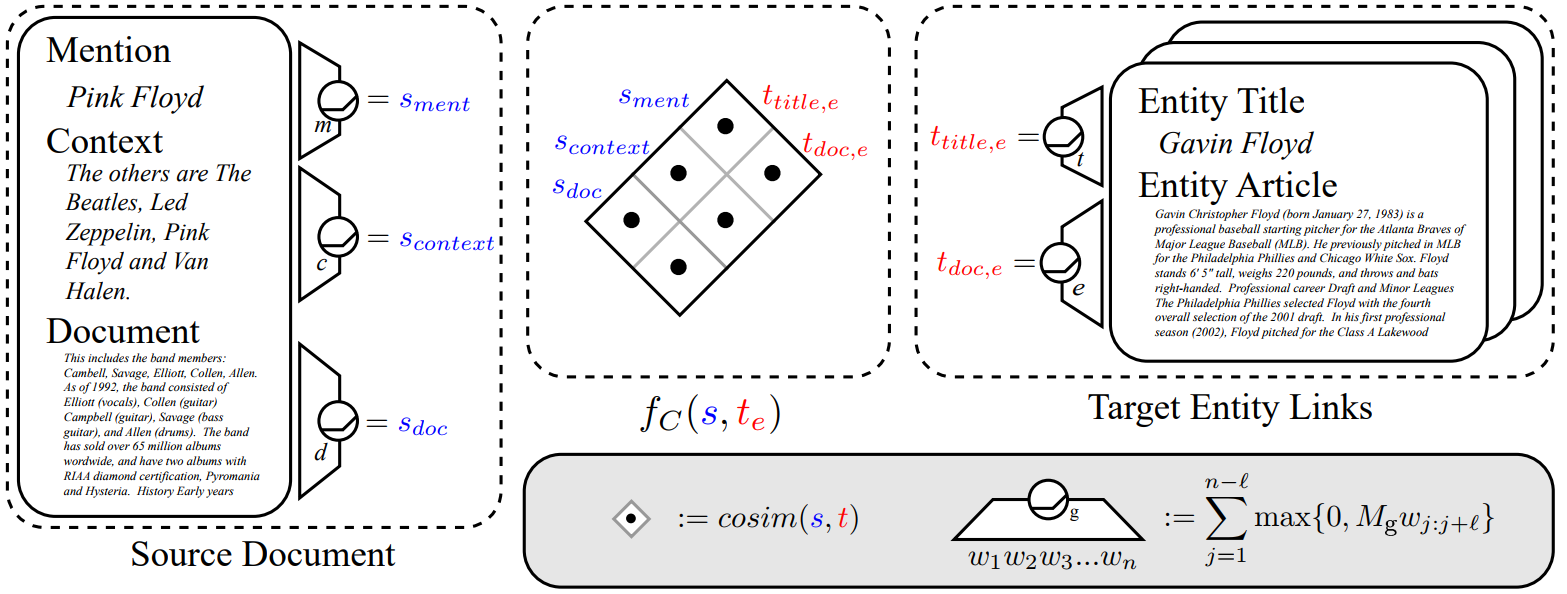
\includegraphics[width=0.95\columnwidth]{figure/rw/linking-francis.png}
	\bicaption{基于多粒度卷积神经网络的实体链接模型。\cite{francis2016capturing}}
    {Entity linking model with CNN at multiple granularities.}
	\label{fig:rw-linking-francis}
\end{figure}


%(68)[Pic][IJCAI] Modeling Mention, Context and Entity with Neural Networks for Entity Disambiguation (TAC-KBP数据集)
Sun等人\cite{sun2015modeling}的模型对不同的上下文信息
采用了不一样的网络结构。
如\figref{fig:rw-linking-sun}所示,
对短语建模的信息包括短语自身,以及去除自身后的句子两部分,
而实体方面,除了利用本身名称之外,还使用了它在维基百科中的分类信息,
用这类人工提炼的知识补充实体的表示。
对句子的表示学习依然使用卷积神经网络,
其余三种信息由于长度较短,均直接使用了词向量平均的方式得到向量表达。
进一步,该模型利用较为复杂的神经张量层将各部分向量结合,
分别得到实体和短语的整体表达。
%以捕捉向量不同维度间的信息交互。
类似的方法还有文献\parencite{gupta2017entity},
对实体的维基分类信息进行表示学习,
通过双向循环神经网络对短语所在句子进行编码。
同时模型定义了不同信息之间的多种损失函数,对训练数据的利用更加充分。
%(7)[Pic][EMNLP] Entity Linking via Joint Encoding of Types, Descriptions, and Context
%(6)[BadPic][COLING] Joint learning of local and global features for entity linking via neural networks (ref充数用,需要再加)

\begin{figure}[th]
	\centering
    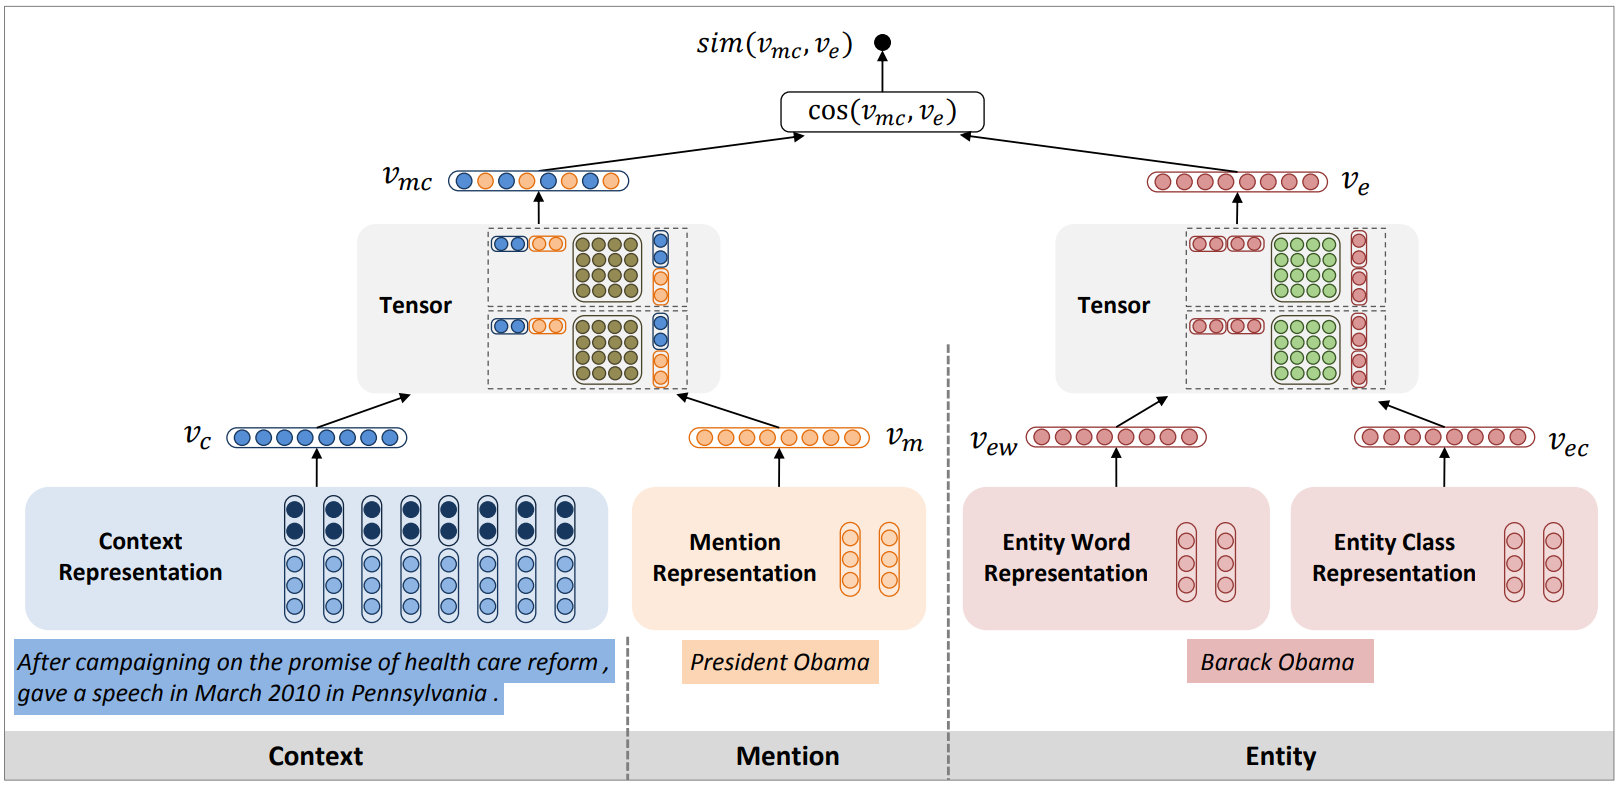
\includegraphics[width=0.95\columnwidth]{figure/rw/linking-sun.png}
	\bicaption{基于神经张量层的链接模型。\cite{sun2015modeling}}{NTN based entity linking model proposed by Sun et al.}
	\label{fig:rw-linking-sun}
\end{figure}

%(22)[NoPic][CoNLL] Entity Disambiguation by Knowledge and Text Jointly Embedding
此外,知识库向量学习技术\cite{bordes2013translating}也被用于实体链接任务中。
知识库向量学习与词向量学习类似,以大量事实三元组作为训练数据,
学习每个实体的向量表示,使得相近语义的实体具有相近的向量。
Fang等人\cite{fang2016entity}提出的链接模型基于知识库向量与词向量的融合:
通过实体与短语互相替代的方式,定义了基于三元组以及共现词对的目标函数,
促使实体与其短语的向量尽可能一致,因此所有向量表示被映射到同一个高维语义空间中。
融合的优势在于实体和单词之间直接可比,
通过距离度量函数计算候选实体与短语上下文中不同词的距离,
并以此作为链接模型的特征。

%(41)[NoPic][CoNLL] Joint Learning of the Embedding of Words and Entities for Named Entity Disambiguation(凑人头)
%(9)[Pic][EMNLP] Deep Joint Entity Disambiguation with Local Neural Attention(凑人头)


%"通过xxx得到xxx,因此可以对xxxx进行建模  进一步xxxx"



%出现在Tutorial里的
%Local and Global Algorithms for Disambiguation to Wikipedia (Ratinov)(Illinois Wikifier)
%Robust Disambiguation of Named Entities in Text (放图)(AIDA数据集)
%Linden: linking named entities with knowledge base via semantic knowledge
%Joint Named Entity Recognition and Disambiguation(EMNLP2015,CRF)(AIDA)
%S-MART(啥数据?)(啥特征?)
%不同特征对应的不同类型。



%\subsection{跨语言场景的实体链接模型}
%\label{sec:rw-linking-bilingual}


\subsection{跨语言词向量}
\label{sec:rw-linking-cle}

上一节的论述中提到了词向量模型,用于学习词汇的连续语义表示,但仅局限于单一语言。
对于涉及多个语言的任务,难点在于如何实现语义的跨语言过渡。
为了解决此问题,跨语言词向量模型(Cross-Lingual Embedding Model)
旨在消除单词语义表示对语言的依赖,
将不同语言的向量表示映射至同一连续空间,并依旧保持相似语义单词更加接近的特性,
以此实现语义迁移。
例如\figref{fig:rw-linking-cle}展示了一个英语和德语之间的共享语义空间,
可以清晰地识别出两种语言间的许多组翻译词对。

\begin{figure}[th]
	\centering
    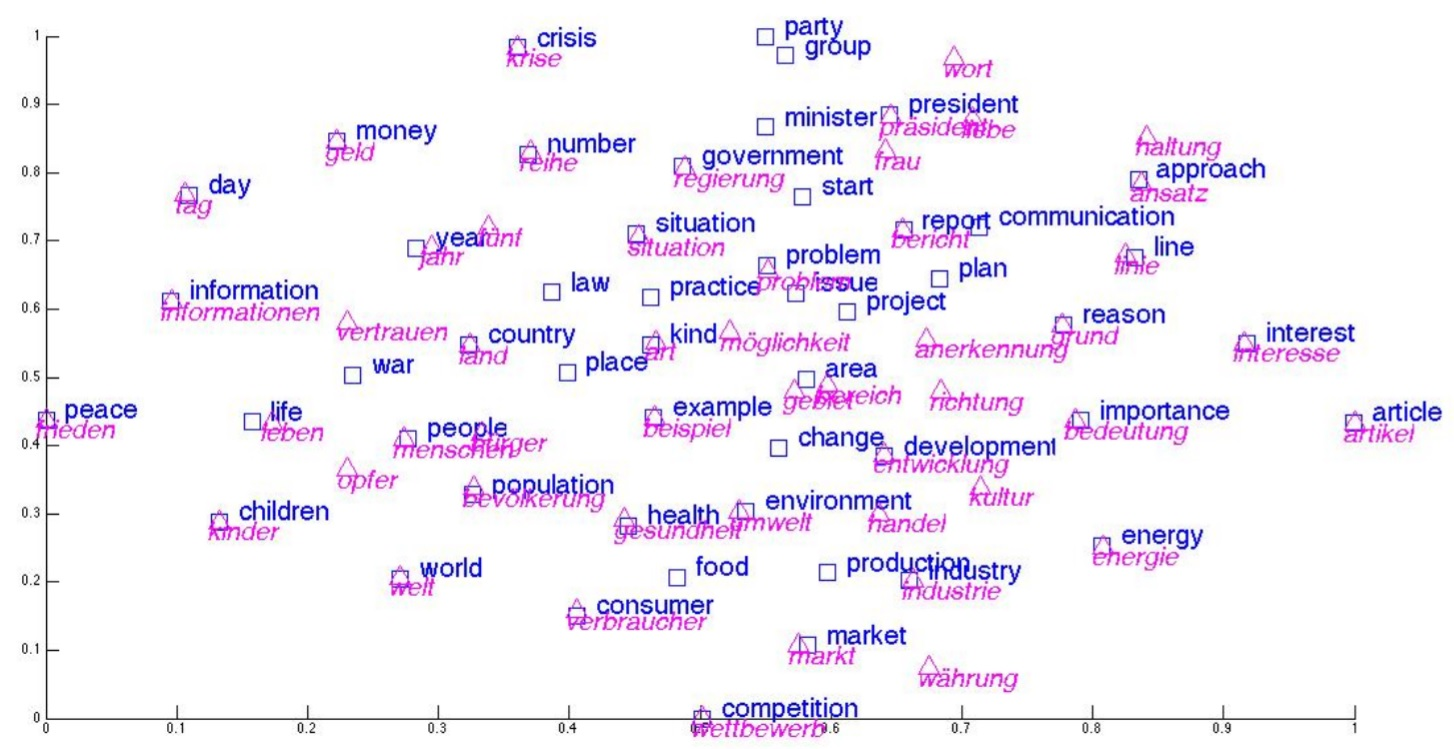
\includegraphics[width=0.8\columnwidth]{figure/rw/linking-cle.jpg}
	\bicaption{英语和德语间的跨语言词向量例子。\cite{ruder2017survey}}
    {An example of cross-lingual word embeddings between English and German.}
	\label{fig:rw-linking-cle}
\end{figure}

跨语言词向量的训练,需要依赖平行语料库用于给模型提供语义对齐信号,
不同的训练方式区别在于平行语料的类型不同,
例如单词级别\cite{mikolov2013exploiting,klementiev2012inducing,lazaridou2015hubness}、
句子级别\cite{hermann2013multilingual,gouws2015bilbowa}、
文档级别\cite{vulic2016bilingual}的对齐。
利用单词级别对齐进行跨语言词向量训练的工作最为普遍,
训练数据主要来自于双语或多语词典中抽取出的高质量翻译词对。
以此为例,对于源语言$s$和目标语言$t$,模型的损失函数$J$由三部分组成:
\begin{equation}
  J = \mathcal{L}_{mono}^{s} + \mathcal{L}_{mono}^{t} + \Omega{}^{s \rightarrow t},
\end{equation}
\noindent
其中,$\mathcal{L}_{mono}$代表各自语言上进行单语言词向量训练的损失,
可直接使用CBOW等已有模型进行计算,
而$\Omega{}^{s \rightarrow t}$为正则项,对应单词对齐的损失。


对于$\Omega{}^{s \rightarrow t}$的定义,相关文献进行了不同的尝试。
Mikolov等人\cite{mikolov2013exploiting}发现,
在不同语言中,多个单词的向量表达之间,几何关系较为相似,
例如英语和西班牙语中,表示数字的单词之间的相对位置几乎一致,
表示动物的单词也有类似特性。
基于以上观察,该工作提出的模型使用了线性变换的方案,
训练转移矩阵$\bm{W}$(或称投影矩阵),
使得源语言词向量$\bm{x}^{s}$经过$\bm{W}$投影后,和对齐的目标语言词向量$\bm{x}^{t}$
的欧氏距离平方(即均方误差)尽可能小:
\begin{equation}
  \Omega{}^{s \rightarrow t} = \sum_i { \| \bm{Wx}_i^s - \bm{x}_{i}^{t}  \|^{2} },
\end{equation}
\noindent
基于线性映射的跨语言词向量模型具有一些变种,
例如文献\parencite{xing2015normalized,zhang2016ten}限制转移矩阵$\bm{W}$为单位正交阵,
以保证映射后的词向量维持单位长度,
Artetxe等人\cite{artetxe2016learning}指出,对于模型效果而言,
转移矩阵正交化比向量正则化更加重要。
Lazaridou等人\cite{lazaridou2015hubness}对$\Omega{}^{s \rightarrow t}$的定义使用了最大间隔(Max Margin)损失
来代替均方误差损失,即不追求$\bm{Wx}^s$与$\bm{x}^t$绝对距离尽可能小,
而是让$\bm{x}^t$比其它任何不相关单词都更加接近$\bm{Wx}^s$,
从而避免跨语言词向量出现过多中枢词的现象。
Faruqui等人\cite{faruqui2014improving}利用
典型相关分析(Canonical Correlation Analysis, CCA)\cite{hotelling1936relations}
进行词向量训练。CCA同为线性投影方式,不同之处在于,
%也可用于将不同语言的词向量线性投影到同一个向量空间中,与之前的线性映射不同,
CCA对两个语言分别学习一个线性变换矩阵,
目标是尽可能降低映射后每个翻译词对的互协方差分值。

%训练过程:分开,joint
%(稍微扯一下优点,虽然还没想好)
此外,跨语言词向量的训练还可
对于通过句子或文档级别的平行语料进行跨语言词向量的训练,由于不是本文的研究重点,
故不展开论述。
跨语言词向量能够应用在多种任务中,
例如文档分类\cite{klementiev2012inducing}、词性标注\cite{zhang2016ten}、
命名实体识别\cite{murthy2016sharing}、机器翻译\cite{zou2013bilingual}等,
其带来的知识迁移具有很高的实用性。
对于训练集和测试集为不同语言的任务,跨语言词向量能实现知识在不同语言上的迁移;
对于类似机器翻译、跨语言实体链接等输入和输出为不同语言的任务,
预训练好的跨语言词向量能够作为特定任务模型的训练起点,
消除语义的间隔,从而提升整体效果。


%Zhang IJCAI 2012 Cross Lingual Entity Linking with Bilingual Topic Model

%Sil AAAI 2018 Neural Cross-Lingual Entity Linking (先放着,来不及了)
%Tsai NAACL 2016 Cross-lingual Wikification Using Multilingual Embeddings (留给小RW)


%Entity linking or wikification is another task tackled using cross-lingual word embeddings
%(Tsai & Roth, 2016). The purpose of the task is to ground mentions written in nonEnglish
%documents to entries in the English Wikipedia, facilitating the exploration and
%understanding of foreign texts without full-fledged translation systems (Ji, Nothman,
%Hachey, & Florian, 2015). Such wikifiers, i.e., entity linkers are a valuable component
%of several NLP and IR tasks across different domains (Mihalcea & Csomai, 2007; Cheng
%& Roth, 2013).






